\subsection{Phân tích phương sai một nhân tố (One-way ANOVA)} \label{anova1}
\subsubsection{Mục đích}
Đánh giá xem biến nhân tố X có ảnh hưởng đến biến phụ thuộc Y hay không? Trong đề tài này chúng ta sẽ kiểm định xem, việc các mùa (season) cũng như hình thức giao hàng nhanh (is\_expedited\_-delivery) sẽ ảnh hưởng như thế nào đến phí giao hàng (delivery\_charges) bằng phương pháp phân tích phương sai ANOVA một nhân tố.
\subsubsection{Tiến hành phân tích}
%yêu mùa ảnh hưởng tới phí giao hàng
Đầu tiên chúng ta sẽ kiểm định xem, việc các mùa (season) ảnh hưởng như thế nào đến phí giao hàng (delivery\_charges) bằng phương pháp phân tích phương sai ANOVA một nhân tố. .Hình \ref{fig:5.1} thể hiện kết quả phân tích phương sai ANOVA một nhân tố cho mẫu thống kê bằng câu lệnh chính là anova1 <- aov(delivery\_charges ~ season, data=loi1) Trong RStudio (xem code từ dòng 381 đến 389 trong file: codeR\_nhom10\_lopTN01.r).
\begin{figure}[!htbp]
    \centering
    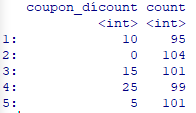
\includegraphics[width=0.5\linewidth]{graphics/5.3.1.png}
    \caption{Phân tích phương sai ANOVA xét sự ảnh hưởng của mùa (season) đến phí giao hàng (delivery\_charges)}
    \label{fig:5.1}
\end{figure}
Quan sát kết quả trên hình \ref{fig:5.1}, giá trị p-value (tức Pr(>F)) là rất rất nhỏ hơn ngưỡng ý nghĩa phổ biến (0.05). Do đó, cho thấy sự khác biệt rất có ý nghĩa thống kê, có đủ bằng chứng thống kê rất mạnh để kết luận rằng, các mùa (season) có ảnh hưởng rất mạnh đến phí giao hàng (delivery\_charges).

Để xác định trung bình của nhóm nào là khác biệt, ta sử dụng phương pháp so sánh bội (Multiple comparison method). Một phương pháp so sánh bội đơn giản và có ý nghĩa độ lệch nhỏ nhất (Least significant difference - LSD) của Fisher. Hình \ref{fig:5.2} thể hiện kết quả của phương pháp so sánh bội Least significant difference - LSD bằng câu lệnh chính là lsd1<- LSD.test(anova1, "season", console=-TRUE) trong thư viện library(agricolae) (xem code dòng 392 trong file: codeR\_nhom10\_lopTN01.r).
\begin{figure}[!htbp]
    \centering
    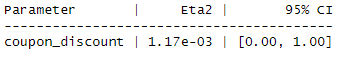
\includegraphics[width=0.6\linewidth]{graphics/5.3.3.png}
    \caption{So sánh bội sau anova của mùa}
    \label{fig:5.2}
\end{figure}

Từ kết quả ở hình trên ta thấy được trung bình, độ lệch chuẩn (Std), số mẫu (r), độ lệch chuẩn trung bình (SE), cận trên của khoản tin cậy (LUL), cận dưới của khoản tin cậy (UCL) đồng thời phân nhóm ý nghĩa. Thông qua phân nhóm ý nghĩa cho thấy mùa thu (Autumn) và mùa đông (Winter) không khác biệt nhau lắm còn mùa hè (Summer) cao hơn và mùa xuân (Spring) là phí giao hàng cao nhất, khác biệt đáng kể nhất so với các mùa còn lại.
%yêu cầu giao hàng nhanh ảnh hưởng tới phí giao hàng

Tiếp theo chúng ta sẽ tiếp tục kiểm định thêm một yếu tố nữa là việc khách hàng yêu cầu giao hàng nhanh (is\_expedited\_delivery) sẽ ảnh hưởng như thế nào đến phí giao hàng (delivery\_charges) bằng phương pháp phân tích phương sai ANOVA một nhân tố. Hình \ref{fig:5.2} thể hiện kết quả phân tích phương sai ANOVA một nhân tố cho mẫu thống kê bằng câu lệnh chính là anova11 <- aov(delivery\_charges ~ is\_expedited\_delivery, data=loi2) Trong RStudio (xem code từ dòng 393 đến 400 trong file: codeR\_-nhom10\_lopTN01.r).
\begin{figure}[!htbp]
    \centering
    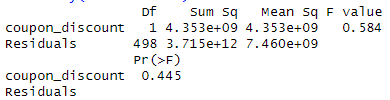
\includegraphics[width=0.6\linewidth]{graphics/5.3.2.png}
    \caption{Phân tích phương sai ANOVA xét sự ảnh hưởng của việc khách hàng yêu cầu giao hàng nhanh (is\_expedited\_delivery) đến phí giao hàng(delivery\_charges)}
    \label{fig:5.3}
\end{figure}
Quan sát kết quả trên hình \ref{fig:5.3}, giá trị p-value (tức Pr(>F)) là rất rất nhỏ hơn ngưỡng ý nghĩa phổ biến (0.05). Do đó, cho thấy sự khác biệt rất có ý nghĩa thống kê, có đủ bằng chứng thống kê rất mạnh để kết luận rằng, việc khách hàng yêu cầu giao hàng nhanh (is\_expedited\_delivery) có ảnh hưởng rất mạnh đến phí giao hàng (delivery\_charges).

Để xác định trung bình của nhóm nào là khác biệt, ta sử dụng phương pháp so sánh bội (Multiple comparison method). Một phương pháp so sánh bội đơn giản và có ý nghĩa độ lệch nhỏ nhất (Least significant difference - LSD) của Fisher. Hình \ref{fig:5.4} thể hiện kết quả của phương pháp so sánh bội Least significant difference - LSD bằng câu lệnh chính là lsd2<- LSD.test(anova11, "is\_expedited\_delivery", console=TRUE)
trong thư viện library(agricolae) (xem code dòng 405 trong file: codeR\_nhom10\_lop-TN01.r)
\begin{figure}[!htbp]
    \centering
    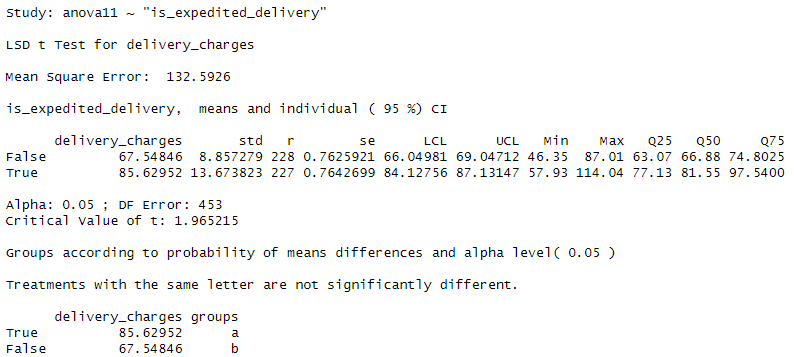
\includegraphics[width=0.6\linewidth]{graphics/5.3.4.png}
    \caption{So sánh bội sau anova của yêu cầu giao hàng nhanh}
    \label{fig:5.4}
\end{figure}

Từ kết quả ở hình trên ta thấy được trung bình, độ lệch chuẩn (Std), số mẫu (r), độ lệch chuẩn trung bình (SE), cận trên của khoản tin cậy (LUL), cận dưới của khoản tin cậy (UCL) đồng thời phân nhóm ý nghĩa. Thông qua phân nhóm ý nghĩa cho thấy việc yêu cầu giao hàng nhanh và không yêu cầu giao hàng nhanh có khác biệt đáng kể.

\subsubsection{Kết luận}
Phân tích ANOVA 1 nhân tố cho thấy season, is\_expedited\_delivery, một cách riêng biệt, có ảnh hưởng đáng kể đến delivery\_charges.